

\begin{frame}{BDT Preselection}
    \begin{itemize}
        \item Channel: 2 tight leptons (e/mu) and 1 (hadronic) tau
        \item Region: n-jets $\ge$ 1 and b-jets $\ge$ 1
        \item Significantly decreasing the dominant Z+jets background
        \item Discrepency due to missing tau fake differentiation
    \end{itemize}
    \begin{figure}
        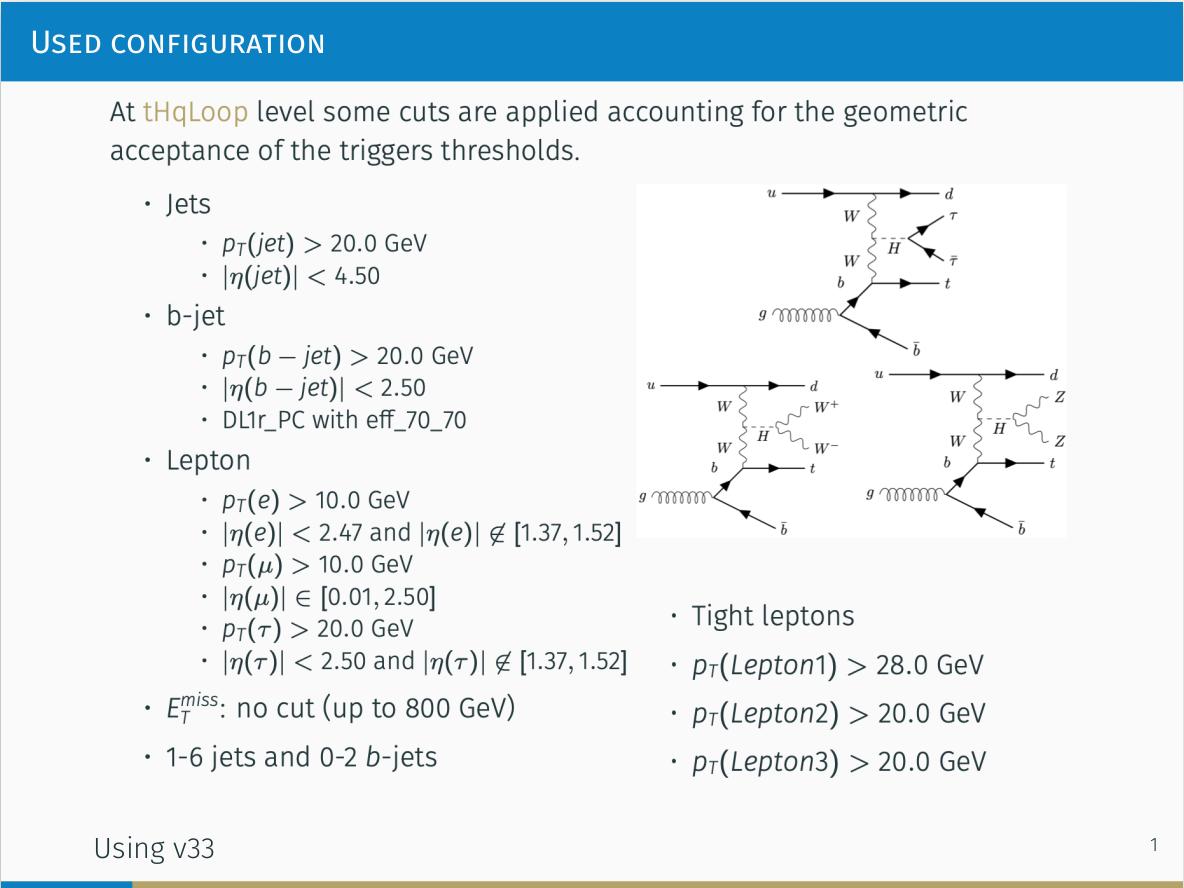
\includegraphics[width=0.7\textwidth]{pablo_selection.png}
    \end{figure}
\end{frame}

\begin{frame}{BDT early results}
    \begin{itemize}
        \item Using XGBoost library
        \item Preliminary: Hyperparameters are not optimised
        \item Visible separation, good training and test agreement
    \end{itemize}
    \begin{columns}
        \begin{column}{0.5\textwidth}
            \begin{figure}
                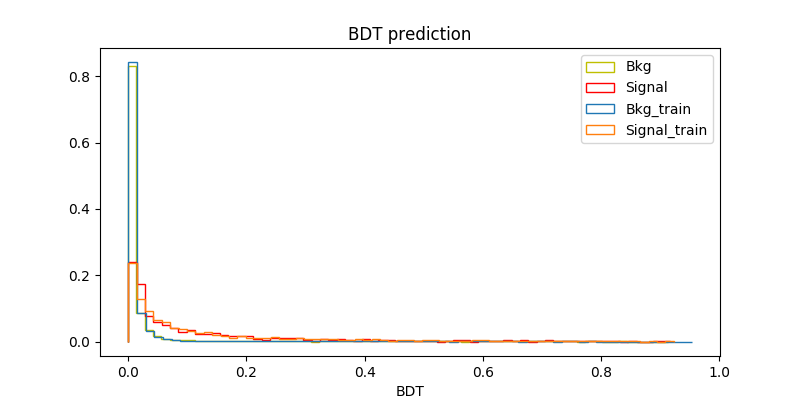
\includegraphics[width=0.9\textwidth]{pablo_response.png}
            \end{figure}           
        \end{column}
        \begin{column}{0.5\textwidth}
            \begin{figure}
                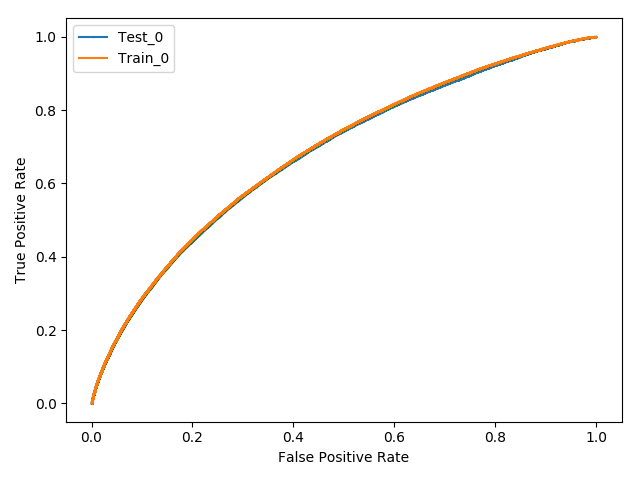
\includegraphics[width=0.9\textwidth]{BDT_ROC.png}
            \end{figure}            
        \end{column}
    \end{columns}

\end{frame}

\begin{frame}{Plan for BDT development}
    \begin{itemize}
        \item {\large BDT hyperparameter tuning}
        \vspace{0.2cm}
        \item {\large Including BDT score in the trees}
        \vspace{0.2cm}
        \item {\large Cut on the BDT score}
        \vspace{0.2cm}
        \item {\large Create a BDT for the CR of the main background}
        \vspace{0.2cm}
        \item Study variables related to SS and OS: Usually, SS and OS have different background contributions.
        \item Get the distributions for forward and central jets separately
    \end{itemize}
\end{frame}